\documentclass[11pt]{article}
\usepackage[margin=1in]{geometry}
\usepackage{clrscode3e}
\usepackage{amsmath,amsthm,amssymb}
\usepackage{mathtools}
\usepackage{tikz}
\usetikzlibrary{positioning,arrows}
%\usepackage{tikz-berge}
%\usepackage{algorithm}
%\usepackage[noend]{algpseudocode}

 
\newcommand{\N}{\mathbb{N}}
\newcommand{\Z}{\mathbb{Z}}
\newcommand{\R}{\mathbb{R}}
\renewcommand{\'}{^{'}}
\renewcommand{\gets}{:=}
 
\newenvironment{theorem}[2][Theorem]{\begin{trivlist}
\item[\hskip \labelsep {\bfseries #1}\hskip \labelsep {\bfseries #2.}]}{\end{trivlist}}
\newenvironment{lemma}[2][Lemma]{\begin{trivlist}
\item[\hskip \labelsep {\bfseries #1}\hskip \labelsep {\bfseries #2.}]}{\end{trivlist}}
\newenvironment{definition}[2][Definition]{\begin{trivlist}
\item[\hskip \labelsep {\bfseries #1}\hskip \labelsep {\bfseries #2.}]}{\end{trivlist}}
\newenvironment{problem}[2][Problem]{\begin{trivlist}
\item[\hskip \labelsep {\bfseries #1}\hskip \labelsep {\bfseries #2.}]}{\end{trivlist}}
\newenvironment{question}[2][Question]{\begin{trivlist}
\item[\hskip \labelsep {\bfseries #1}\hskip \labelsep {\bfseries #2.}]}{\end{trivlist}}

\begin{document}
\title{Chapter 1}
\author{Zachary Campbell}

\maketitle

\begin{section}{Bipartite graphs and matchings}

	Throughout this thesis we will be interested in a specific subclass of graphs known as 
	bipartite graphs. Unless otherwise noted, our algorithms will assume a bipartite structure.

	\begin{definition}{(Bipartite graph)}
		A \emph{bipartite graph} is a graph whose vertices can be partitioned into two 
		sets $L$ and $R$ such that all edges connect a vertex $l\in L$ to a vertex $r\in R$.
		We will denote this graph $G = (L,R,E)$, where $E$ is the edge set.
	\end{definition}
	
	\begin{figure}[h]
		\centering
	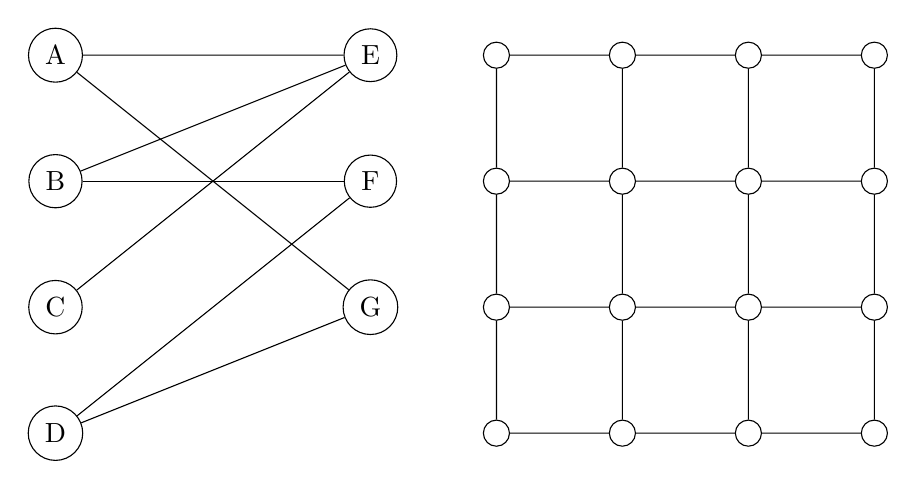
\begin{tikzpicture}[scale=.8,auto=left,every node/.style={circle,draw=black}]
		%left nodes
		\node (n1) at (1,10) {A};
		\node (n2) at (1,8) {B};
		\node (n3) at (1,6) {C};
		\node (n4) at (1,4) {D};

		%right nodes
		\node (n5) at (6,10) {E};
		\node (n6) at (6, 8) {F};
		\node (n7) at (6, 6) {G};
		
		%edges
		\draw (n1) -- (n5);
		\draw (n1) -- (n7);
		\draw (n2) -- (n5);
		\draw (n2) -- (n6);
		\draw (n3) -- (n5);
		\draw (n4) -- (n6);
		\draw (n4) -- (n7);

		%left nodes
		\node (n1) at (8,10) {};
		\node (n2) at (8,8) {};
		\node (n3) at (8,6) {};
		\node (n4) at (8,4) {};

		%center left nodes
		\node (n5) at (10,10) {};
		\node (n6) at (10,8) {};
		\node (n7) at (10,6) {};
		\node (n8) at (10,4) {};

		%center right nodes
		\node (n9) at (12,10) {};
		\node (n10) at (12,8) {};
		\node (n11) at (12,6) {};
		\node (n12) at (12,4) {};

		%right nodes
		\node (n13) at (14,10) {};
		\node (n14) at (14,8) {};
		\node (n15) at (14,6) {};
		\node (n16) at (14,4) {};

		%edges
		\draw (n1) -- (n2);
		\draw (n1) -- (n5);
		\draw (n2) -- (n3);
		\draw (n2) -- (n6);
		\draw (n3) -- (n4);
		\draw (n3) -- (n7);
		\draw (n4) -- (n8);
		\draw (n5) -- (n6);
		\draw (n5) -- (n9);
		\draw (n6) -- (n7);
		\draw (n6) -- (n10);
		\draw (n7) -- (n8);
		\draw (n7) -- (n11);
		\draw (n8) -- (n12);
		\draw (n9) -- (n10);
		\draw (n9) -- (n13);
		\draw (n10) -- (n11);
		\draw (n10) -- (n14);
		\draw (n11) -- (n12);
		\draw (n11) -- (n15);
		\draw (n12) -- (n16);
		\draw (n13) -- (n14);
		\draw (n14) -- (n15);
		\draw (n15) -- (n16);
	\end{tikzpicture}
	\caption{Examples of bipartite graphs}
	\end{figure}

	In Figure 1 we have a bipartite graph with vertex partition given by $L = \{A,B,C,D\}$ and 
	$R = \{E,F,G\}$. All edges in this graph are between a node $l\in L$ and a node $r\in R$. The 
	graph on the right is also bipartite. It may take a little more time to convince yourself that 
	you can partition the vertices into disjoint $L$ and $R$ in a way that maintains the 
	bipartite property. Try it!

	Now that we know what we are working with, let's introduce a problem that 
	we'd like to solve on these graphs.
	We now describe the notion of a matching on a graph.  


	\begin{definition}{(Matching)}
		Let $G = (V,E)$ be a graph. A subset $M\subset E$ is a \emph{matching} if no two 
		edges in $M$ are incident to the same vertex.
	\end{definition}

	We say that a vertex $v\in V$ is matched with respect to $M$ if it is an endpoint of some 
	edge in $M$. The following figure shows some examples of different matchings on one of the 
	graphs from Figure 1.

	\begin{figure}[h]
		\centering
		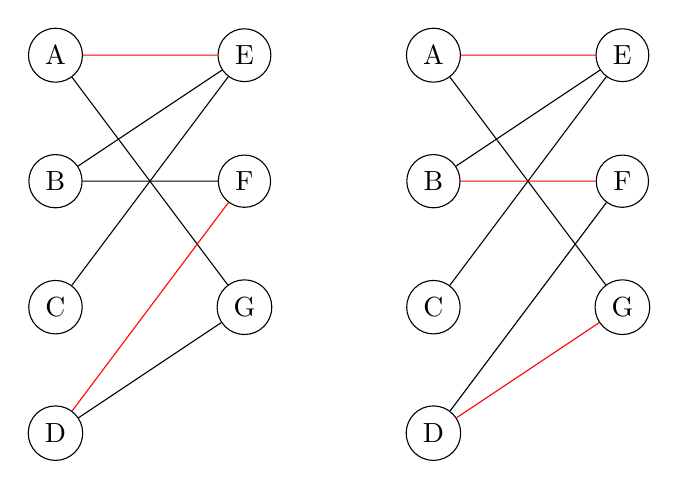
\begin{tikzpicture}[scale=.8,auto=left,every node/.style={circle,draw=black}]
		
		%left nodes
		\node (n1) at (1,10) {A};
		\node (n2) at (1,8) {B};
		\node (n3) at (1,6) {C};
		\node (n4) at (1,4) {D};

		%right nodes
		\node (n5) at (4,10) {E};
		\node (n6) at (4, 8) {F};
		\node (n7) at (4, 6) {G};
		
		%edges
		\draw[red] (n1) -- (n5);
		\draw (n1) -- (n7);
		\draw (n2) -- (n5);
		\draw (n2) -- (n6);
		\draw (n3) -- (n5);
		\draw[red] (n4) -- (n6);
		\draw (n4) -- (n7);

		%left nodes
		\node (m1) at (7,10) {A};
		\node (m2) at (7,8) {B};
		\node (m3) at (7,6) {C};
		\node (m4) at (7,4) {D};

		%right nodes
		\node (m5) at (10,10) {E};
		\node (m6) at (10, 8) {F};
		\node (m7) at (10, 6) {G};
		
		%edges
		\draw[red] (m1) -- (m5);
		\draw (m1) -- (m7);
		\draw (m2) -- (m5);
		\draw[red] (m2) -- (m6);
		\draw (m3) -- (m5);
		\draw (m4) -- (m6);
		\draw[red] (m4) -- (m7);

		\end{tikzpicture}
		\caption{Examples of matchings on a bipartite graph}
	\end{figure}

	There many different valid matchings on the graph in Figure 2. Oftentimes, we want to find 
	the largest matching on a graph. (ADD SENTENCE OR TWO ON MOTIVATION FOR MAXIMAL MATCHING.)
	This leads to the following definition.

	\begin{definition}{(Maximal matching)}
		A \emph{maximal matching} on $G$ is a matching $M$ such that if any other edge 
		not in $M$ is added to $M$, it is no longer a valid matching. Alternatively put, 
		$M$ is maximal if there is no matching $M\'$ such that $M\subset M\'$.
	\end{definition}

	Both matchings in Figure 2 are maximal matchings; in each case there are no edges that 
	we can add to $M$ and have that $M$ is still a matching. However, notice that the size of 
	the matchings is different, even though both are maximal on $G$. This leads to the following 
	definition.

	\begin{definition}{(Maximum matching)}
		A matching $M$ on a graph $G$ is said to be a maximum matching if for all other 
		matchings $M\'$ on $G$, $|M\'| \leq |M|$.
	\end{definition}

	In our example, the matching on the right given by $M = \{(A,E), (B,F), (D,G)\}$ is a 
	maximum matching (convince yourself). In general there may be many unique maximum matchings 
	on a graph.\\
	In this section we are interested in general methods for finding maximum matchings on 
	bipartite graphs. One of the fundamental approaches is to look at certain subgraphs called 
	alternating paths. Before we define what these are, let's look at a motivating example.
	Suppose we have the matching on the left in Figure 2. So $M = \{(A,E),(D,F)\}$. Consider 
	the following sequence of vertices in the graph:

	\begin{figure}[h]
		\centering
		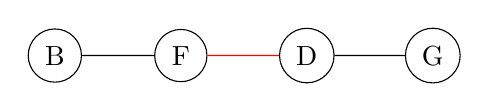
\begin{tikzpicture}[scale=.8,auto=left,every node/.style={circle,draw=black}]

			\node (n1) at (1,10) {B};
			\node (n2) at (3,10) {F};
			\node (n3) at (5,10) {D};
			\node (n4) at (7,10) {G};

			\draw (n1) -- (n2); 
			\draw[red] (n2) -- (n3);
			\draw (n3) -- (n4);
		\end{tikzpicture}
	\end{figure}

	Call this sequence $p$. Let's perform an 
	operation that we will denote $M\oplus p$, which operates like XOR: add to $M$ each edge in 
	$p$ that isn't in $M$, and remove from $M$ each edge in $p$ that is in $M$. This gives us 
	the following segment, where $(B,F)$ and $(D,G)$ are now in $M$, but $(D,F)$ is not:

	\begin{figure}[h]
		\centering
		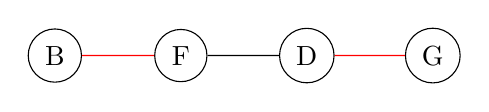
\begin{tikzpicture}[scale=.8,auto=left,every node/.style={circle,draw=black}]

			\node (n1) at (1,10) {B};
			\node (n2) at (3,10) {F};
			\node (n3) at (5,10) {D};
			\node (n4) at (7,10) {G};

			\draw[red] (n1) -- (n2); 
			\draw (n2) -- (n3);
			\draw[red] (n3) -- (n4);
		\end{tikzpicture}
	\end{figure}

	First, we must check that the new $M$ is still a valid matching; we do this by noticing that 
	$B$ and $G$ were originally unmatched, so it's okay for one of their incident edges to be 
	added. Also, notice that the size of our matching has grown by 1! In fact, this new matching 
	is exactly the matching given by the graph on the right in Figure 2. 
	This is a general technique in 
	finding maximum matchings. We want to look for these paths that start and end at unmatched 
	vertices, and whose edges are alternately matched and unmatched. If we can find one of these 
	paths, we will be able to increase the size of matching. We define this formally now.

	\begin{definition}{(Alternating path)}
		Let $G$ be a graph and $M$ some matching on $G$. An \emph{alternating path} is a 
		sequence of vertices and edges that begins with an unmatched vertex, and whose 
		edges alternate between being in $M$ and not in $M$.
	\end{definition}

	\begin{definition}{(Augmenting path)}
		An \emph{augmenting path} is an alternating path that starts and ends on unmatched 
		vertices. When we augment $M$ by an augmenting path $p$, we use the notation 
		$M\oplus p$.
	\end{definition}

	This motivates a general method for finding a maximum matching on a bipartite graph: 
	just keep looking for augmenting paths, and augment the current matching by that augmenting 
	path. Of course, we need to prove that this in fact gives us a maximum matching. The following 
	theorem says exactly that.

	\begin{theorem}{(Berge, 1957)}
		A matching $M$ on $G$ is a maximum matching if and only if $G$ contains no augmenting 
		paths with respect to $M$.
	\end{theorem}

	This gives us the following framework for finding maximum matchings in bipartite graphs.

	\begin{codebox}
		\Procname{$\proc{Alg 1} (G) $}
		\li $M \gets \emptyset $
		\li $\While$ there exists an augmenting path $p$
			\Do
		\li		$M \gets M\oplus p$
			\End
		\li $\Return$ $M$
	\end{codebox}

	Note that we have yet to describe the details of this algorithm. Before we do so, we are going 
	to take a step back a bit and look at the maximum matching problem from a slightly different 
	perspective. In doing so, we will develop a language for talking about this problem that will 
	serve us throughout the rest of this thesis. At first, the approach will appear purely 
	pedagogic, but hopefully the reader will understand the significance of it by the end of the 
	thesis.

\end{section}

\begin{section}{The vertex cover problem}
	We begin this section by defininig a new problem. Again, this is a problem on graphs in 
	general, but we will be restricting our attention to bipartite graphs. This is a good idea 
	for many reasons, but the most pertinent reason is that this problem is NP-complete in the 
	general case.

	\begin{definition}{(Vertex cover)}
		Let $G = (L,R,E)$ be a bipartite graph. A subset $C\subset L\cup R$ is said to be a 
		\emph{vertex cover} if for each $(i,j)\in E$ is such that at least one of $i,j \in C$.
		$C$ is a \emph{minimum} vertex cover if for any other cover $C\'$, $|C|\leq |C\'|$.
	\end{definition}

	Using what we've already learned, we can specify at least one relation between matchings and 
	vertex covers: namely, the vertices of all edges in any maximal matching on a graph forms a 
	vertex cover. Here are some examples of vertex covers on the graph we've been looking at.

	\begin{figure}[h]
		\centering
		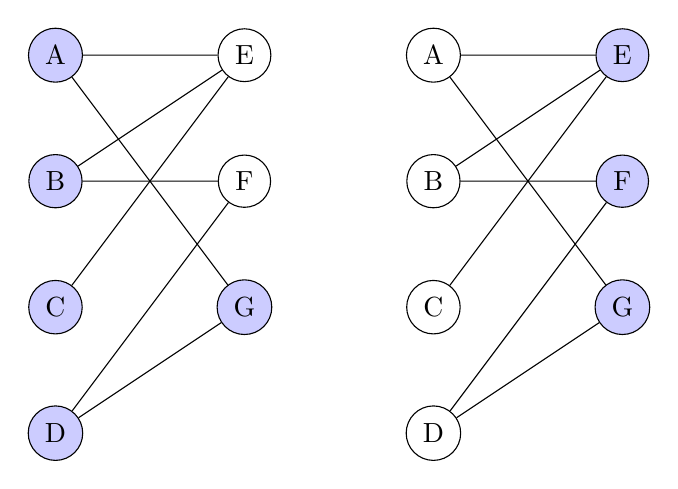
\begin{tikzpicture}[scale=.8,auto=left,every node/.style={circle,draw=black}]
		
		%left nodes
		\node[fill=blue!20] (n1) at (1,10) {A};
		\node[fill=blue!20] (n2) at (1,8) {B};
		\node[fill=blue!20] (n3) at (1,6) {C};
		\node[fill=blue!20] (n4) at (1,4) {D};

		%right nodes
		\node (n5) at (4,10) {E};
		\node (n6) at (4, 8) {F};
		\node[fill=blue!20] (n7) at (4, 6) {G};
		
		%edges
		\draw (n1) -- (n5);
		\draw (n1) -- (n7);
		\draw (n2) -- (n5);
		\draw (n2) -- (n6);
		\draw (n3) -- (n5);
		\draw (n4) -- (n6);
		\draw (n4) -- (n7);

		%left nodes
		\node (m1) at (7,10) {A};
		\node (m2) at (7,8) {B};
		\node (m3) at (7,6) {C};
		\node (m4) at (7,4) {D};

		%right nodes
		\node[fill=blue!20] (m5) at (10,10) {E};
		\node[fill=blue!20] (m6) at (10, 8) {F};
		\node[fill=blue!20] (m7) at (10, 6) {G};
		
		%edges
		\draw (m1) -- (m5);
		\draw (m1) -- (m7);
		\draw (m2) -- (m5);
		\draw (m2) -- (m6);
		\draw (m3) -- (m5);
		\draw (m4) -- (m6);
		\draw (m4) -- (m7);

		\end{tikzpicture}
		\caption{Examples of vertex covers}
	\end{figure}

	You can convince yourself that the cover on the right is a minimum cover. This brings us 
	to an important theorem. We first prove a lemma.

	\begin{lemma}{1}
		Let $G=(L,R,E)$ be a bipartite graph. Let $M$ be a matching on $G$ and $C$ a cover on 
		$G$ such that $|M| = |C|$. Then $M$ is a maximum matching and $C$ is a minimum 
		covering.
	\end{lemma}

	\begin{proof}
		Let $M\'$ be a maximum matching on $G$ and $C\'$ a minimum covering on $G$. For each 
		$(i,j)\in M\'$, $C\'$ must include either $i$ or $j$, which tells us that 
		$|M\'| \leq |C\'|$. Then we have 
		\[
			|M|\leq |M\'| \leq |C\'| \leq |C|.
		\]
		Thus, if $|M| = |C|$ we have equalities above, which means that the size of a maximum 
		matching is equal to the size of a minimum covering.
	\end{proof}

	Before we prove this, we define a couple of terms. Given a matching $M$, we say a vertex is 
	\emph{saturated} if it is incident to some edge in $M$. Also, an $M$-alternating path is 
	an alternating path with respect to $M$.

	\begin{theorem}{(K\H{o}nig-Egervary)}
		For any bipartite graph $G$, if $M$ is a maximum matching on $G$ and $C$ is a minimum 
		vertex cover  on $G$, then $|M| = |C|$.
	\end{theorem}

	\begin{proof}
		Let $G=(L,R,E)$ be a bipartite graph, and let $M$ be a maximum matching on $G$. 
		Furthermore, define
		\[
			A := \{s\in S\; |\; s \text{ unsaturated}\}
		\]
		and
		\[
			B := \{\text{all vertices connected to nodes in $A$ by $M$-alternating paths}\}
			.
		\]
		Let $U = B\cap L$ and $V = B\cap R$. Then we have the following:

		\begin{enumerate}
			\item Every node in $V$ is saturated.
			\item $N(U) = V$,
		\end{enumerate}

		where $N(U)$ denotes the set of all vertices connected to elements of $U$ (the 
		``neighbors'' of $U$). The first claim comes from the fact that, if $M$ is a 
		maximum matching, then our alternating paths starting at nodes in $A$ must have 
		length $\geq 2$, and must have even length (otherwise we would have an augmenting path, 
		which contradicts our assumption that $M$ is a maximum matching).
		The second comes from that fact that every node in $N(U)$ is connected to vertices in 
		$A$ by an alternating path. \\
		Now, define $K := (L\setminus U)\cup V$. Every edge 
		in $G$ must have one of its endpoints in $K$. If not, there there would be an 
		edge with one end in $U$ and one end in $R\setminus V$, which contradicts 
		$N(U) = V$. So $K$ is a covering of $G$. Moreover, $|K| = |M|$, since for each 
		edge in $M$ we've included one of its endpoints in $K$ (the vertices we've chosen are 
		those in $N(U)$ and those in $L\setminus U$). Thus, by the previous lemma, $K$ is 
		a minimum covering.
	\end{proof}

	All of this tells us that there is a deep relationship between maximum matchings and 
	minimum vertex covers on bipartite graphs. Given a solution to one, we can turn it into a 
	solution to the other. This is what we seek to accomplish next. 
\end{section}

\begin{section}{Linear programming}
	Add sentence relating to last section (we are formulating this things as optimization problems).
	For a more detailed treatment on linear programming, we will refer you to (CITE LP SOURCES).
	For the purposes of this thesis, we will treat linear programming more casually, only requiring 
	few key results. Moreover, we will not be discussing methods of actually solving linear 
	programs. \\
	In the general linear-programming problem, our goal is to optimize some linear function that 
	is constrained by a set of linear inequalities. These problems are ubiquitous in applied math 
	and computer science, as they model a system in which something needs to be optimized according 
	to competing resources. We can express a general \emph{maximization} linear program as

	\begin{alignat}{3}
		& \text{maximize } & \sum_{j=1}^{n} c_{j} x_{j}& \\
		& \text{subject to } \quad & \sum_{j=1}^{n} a_{ij} x_{j} & \leq b_{j}, & i & = 1, \dots 
		, m \\
				&& x_{j} & \geq 0, \quad & j & = 1, \dots, n.
	\end{alignat}
	We call the function in (1) our \emph{objective function}, and the linear inequalities (2) and 
	(3) our constraints. Similarly, a \emph{minimization} linear program takes the form

	\begin{alignat}{3}
		& \text{minimize } & \sum_{j=1}^{n} c_{j} x_{j}& \\
		& \text{subject to } \quad & \sum_{j=1}^{n} a_{ij} x_{j} & \geq b_{j}, & i & = 1, \dots 
		, m \\
				&& x_{j} & \geq 0, \quad & j & = 1, \dots, n.
	\end{alignat}
	Many problems which on the face may not appear to be optimization problems turn out to be 
	easily rephrased as linear programs. Our goal in this section will 
	be to describe our two problems, maximum matchings and minimum vertex covers, as linear 
	programs. Before doing so, we describe duality theory, which allows us to draw relationships 
	between certain linear programs.\\

	Duality theory gives us a way to prove bounds on optimal solutions to linear programs. We first 
	define the dual of a linear program.

	\begin{definition}{(Dual)}
		Let 
		\begin{alignat*}{2}
			& \text{maximize} & \mathbf{c}^{T}\mathbf{x} \\
			& \text{subject to } & A\mathbf{x} & \leq \mathbf{b} \\
			&& \mathbf{x} &\geq 0
		\end{alignat*}

		be our linear program, which we will call the \emph{primal} linear program. Then we 
		define the \emph{dual} of this linear program to be the linear program
		\begin{alignat*}{2}
			& \text{minimize} & \mathbf{b}^{T}\mathbf{y} \\
			& \text{subject to } & A^{T}\mathbf{y} & \leq \mathbf{c} \\
			&& \mathbf{y} &\geq 0
		\end{alignat*}
	\end{definition}
	The first thing to note is that the dual of the dual is the primal. Let us introduce some 
	notation. First, let us denote the primal maximization problem by the letter $\Gamma$, and 
	the dual minimization problem by the letter $\Omega$. For a given linear program, we denote 
	an optimal solution by $\mathbf{OPT}$. 
	%%add bit on notation on capital greek letters, OPT, etc so this is clear%%

	\begin{theorem}{(Weak duality)}
		If the primal linear program (in maximization form) and the dual (in minimization 
		form) are both feasible, then 
		\[
			\mathbf{OPT}(\Gamma) \leq \mathbf{OPT}(\Omega).
		\]
	\end{theorem}
	What's surprising is the following theorem.

	\begin{theorem}{(Strong duality)}
		Given two linear programs $\Gamma$ and $\Omega$ that are duals of each other, if one is 
		feasible and bounded, then so is the other. Additionally, 
		\[
			\mathbf{OPT}(\Gamma) = \mathbf{OPT}(\Omega).
		\]
	\end{theorem}
	Our goal now is to use this theory to relate the maximum matching problem to the minimum 
	vertex cover problem.\\

	Let's first turn maximum matching into a linear program. Our goal is to maximize the number 
	of edges in our matching. Our constraint is that no edge is incident to more than one edge 
	in the matching. So for each edge $(i,j)$, we will need a corresponding $x_{ij}$. Our objective 
	function is then pretty simple: maximize the number of $x_{ij}$. Now we need to figure out 
	our constraint equations. For a fixed node $i$, the number of edges in the matching incident 
	to $i$ is given by $\sum_{j} x_{ij}$. So we want that this is $\leq 1$. Similarly, for any 
	node $j$, we want $\sum_{i} x_{ij} \leq 1$. This gives us the following linear program.

	%Maximum matching ILP%

	\begin{alignat}{3}
		& \text{maximize } & \sum_{i,j} x_{ij}& \\
		& \text{subject to } \quad & \sum_{j} x_{ij} & \leq 1, & \quad \forall i\in S&, \\
				     &\quad & \sum_{i} x_{ij} & \leq 1, & \quad \forall j\in T &, \\
				&& x_{ij} & \in \{0,1\}.
	\end{alignat}
	Now let's try and construct the dual of this linear program. We will need a variable 
	$u_i$ for each vertex $i$ in (8). Similarly, we need a variable $v_j$ for each vertex $j$ in 
	(9). Our objective will be to minimize over the sum of these $u_i,v_j$. Since our constraint 
	in the primal is the constant vector 1, our only constraint will be that $u_i + v_j \geq 1$. 
	This gives us the dual linear program

	%Vertex cover ILP%

	\begin{alignat}{3}
		& \text{minimize } & \sum_{i,j} (u_i + v_j)& \\
		& \text{subject to } \quad & u_i + v_j & \geq 1 & \quad \forall i,j &, \\
				    && u_i,v_j & \in \{0,1\}.
	\end{alignat}

	%note that i've shown only integer linear programs, talk about non-integer LPs%%

	This dual problem tells us that each edge must be ``covered'' by at least one of its incident 
	vertices. This is exactly the vertex cover problem! So for bipartite graphs, the linear 
	programs for maximum matchings and minimum vertex covers are duals of each other. We will 
	use this insight to construct our algorithms for solving the maximum matching problem.\\	
\end{section}

\begin{section}{Primal-dual matching algorithms}

	The reader may be familiar with matching algorithms via Ford-Fulkerson. They likely took a 
	flow approach to the problem. Here, we take an approach motivated by the integer linear 
	programs we described in the previous section. 

	\begin{definition}{(Alternating tree)}
		Let $G = (L,R,E)$ be a bipartite graph, and $M$ a matching on $G$. An 
		\emph{alternating tree} with respect to $M$ is a tree which satisfies two 
		conditions:
		\begin{itemize}
			\item the tree contains exactly one node $i\in L$. We call $i$ the 
				\emph{root} of the tree.
			\item all paths between the root and any other node in the tree are 
				alternating paths.
		\end{itemize}
	\end{definition}
	
	The K\H{o}nig Egervary theorem provides much of the motivation for this algorithm. Given a 
	maximum matching, it tells us how to construct a minimum vertex cover. As this is a primal dual 
	algorithm, we will be simultaneously constructing a maximum matching and a minimum vertex 
	cover. Additionally, we want to maintain primal-dual feasibility at all steps in the 
	computation. 
	We initialize with the feasible matching $M = \emptyset$. Let's figure out what to initialize 
	our vertex cover as. The most straightforward thing to do would be to initialize our vertex 
	cover as $L\cup R$. This is certainly a feasible vertex cover, and a strict upper bound on 
	the size of all other vertex covers. However, it turns out we can do a little better than 
	this. Using the K\H{o}nig-Egervary theorem and the weak duality theorem, let's construct 
	an initial vertex cover based on the intial matching $M = \emptyset$. Using the notation 
	from the K\H{o}nig-Egervary theorem, our set $A = L$, since all vertices in $L$ are 
	unsaturated. Then our set $B = L\cup R$. Thus, our set $K$ is equal to $R$. So we can set our 
	initial vertex cover $C = R$. Note that this is a tighter upper bound on the size of vertex 
	covers.
	The algorithm looks at exposed nodes in $L$, and seeks augmenting paths from that node. In this 
	way, each exposed $i\in L$ becomes the root of an alternating tree. Additionally, each time 
	we augment, we update the information regarding our cover. This means we update the sets 
	$A$ and $B$, (and thus $U$, $V$, and $C$). 
	In order to explicitly state how we augment, we will associate with each vertex $k$ a label 
	$\pi_{k}$, which is equal to $\emptyset$ for exposed vertices in $L$; for vertices $j$ in $T$ 
	that are exposed, their label will be equal to some vertex $i\in L$ where $(i,j)\in E$ and 
	$(i,j)\notin M$. We use these labels to trace the alternating path all the way to the source, 
	which will have label $\emptyset$.
	\begin{codebox}
		\Procname{$\proc{ALG 2}\ (G=(L,R,E))$}
		\li $M \gets \emptyset$
		\li $A \gets L$, $B \gets L\cup R$, $C\gets R$
		\li \While $|M| < |C|$
			\Do
		\li		\For $i\in L$ with label $\emptyset$
					\Do
		\li				\For $(i,j)\notin M$
							\Do
		\li						label $\pi_{j} \gets i$ unless already 
								labeled`
							\End
					\End
		\li		\For $j\in R$
					\Do
		\li				\If $j$ is exposed
							\Then
		\li						augment
		\li						update $A$, $B$, $C$
		\li						remove all labels on vertices
		\li						label each exposed $i\in L$ with 
								$\emptyset$
							
		\li					\Else
		\li						find the unique $(i,j)\in M$, label 
								$\pi_{i} \gets j$.
						\End
					\End
			\End
		\li \Return $M$ and $C$
	\end{codebox}
	We know what an augmenting path means in the primal: our sum $\sum_{i,j} x_{ij}$ increases by 
	one. But how can we interpret augmenting paths from the dual perspective? We know that it 
	decreases the size of the set $A$ by one. 



\end{section}



\end{document}
